% File SDSS2020_SampleExtendedAbstract.tex
\documentclass[10pt]{article}
\usepackage{sdss2020} % Uses Times Roman font (either newtx or times package)
\usepackage{url}
\usepackage{latexsym}
\usepackage{amsmath, amsthm, amsfonts}
\usepackage{algorithm, algorithmic}  
\usepackage{graphicx}
\usepackage{lipsum}
\usepackage{enumerate}
\usepackage{indentfirst}
\title{Athernet: Acoustic-based User Space Network Stack} 

\author{
  Cheng Peng \\
   ShanghaiTech University   \\
  {\tt pengcheng2@shanghaitech.edu.cn} \\\And
 Huizhe Su \\
   ShanghaiTech University  \\
  {\tt suhzh@shanghaitech.edu.cn} \\}
  

\date{\today}

\begin{document}
\maketitle
\begin{abstract}
  Athernet is a user-space TCP/IP stack with full functionality and handy utilities built on the acoustic channel. This report describes the main architecture design and the technical implementation of the Athernet.
\end{abstract}

{\bf Keywords:} network stack, acoustic link, network protocol
\section{Introduction}
\lipsum[1-2]

\section{Data Link}
The foundation of the entire network stack is the data link layer which
provides reliable bidirectional packet transmission between two nodes in a shared noisy acoustic medium.
The data link layer consists of the physics sublayer and the medium access control sublayer.

\subsection{Physics Sublayer (PHY)}
Bulit on the audio I/O library, PHY enables basic data transmission with no delivery or integrity guarantee.
A PHY frame is a sequence of PCM audio signal samples that represents a chunk of bytes. It is the transmission unit on this layer.
Each frame contains a fixed preamble signal at the beginning for detection as well as synchronization and a payload signal that encodes 0/1 bits.\par
For data transmission, PHY layer constructs a frame from a chunk of bytes and send it through the medium.
For data receiving, PHY layer repeatedly pulls audio samples from the medium and seek for PHY frame based on the frequency-domain feature of the preamble.
When a frame is identified, the payload signal is extracted and decoded.
\subsubsection{Preamble Signal Design}
A chirp is a signal whose instaneous frequency increases or decreases with time.
$x_p(t)$ is a linear chirp signal whose lowest and highest instaneous frequency are $f_a$ and $f_b$ respectively.
\[
	x_p(t) = \begin{cases}
		\pi \dfrac{f_b-f_a}{T} t^2       + 2\pi f_a t     & t\in [0,T]  \\
		\pi \dfrac{f_a-f_a}{T} {(t-T)}^2 + 2\pi f_b (t-T) & t\in [T,2T]
	\end{cases}
\]
For 48kHZ sampling frequency, we choose a up-down chirp where $(f_a,f_b)=

\subsubsection{Modulation and Demodulation}
In order to transmit and receive digital signals, a modulation scheme has to be implemented.
\par
For wireless scenario, strong background noisy is detected from 0Hz to 6000Hz,
so a passband modulation scheme
combining binary phase shift keying (BPSK) and orthogonal frequency-division multiplexing (OFDM)
is implemented.
BPSK encodes bits with phase changes:
\begin{align*}
	x_0(t) & =\sin(2\pi f\, t)
	x_1(t) & =\sin(2\pi f\, t + \pi) = -\sin(2\pi f)
\end{align*}
are used to represent 0 bit and one 1 respectively.
The physics layer sends a bit by pushing samples of the modulated signal to audio I/O driver.
To recover a bit from audio signal, physics layer calculates the dot product of the receive samples and the samples of $x_0(t)$.
\[
	x_0(t)\cdot x_0(t) > 0
	\quad
	x_0(t)\cdot x_1(t) < 0
\]
A zero bit is produced if the dot product is positive, otherwise a one bit is produced.

As for cabel-connected scenario, baseband transmission is possible as low frequency background noise has less power compared with wireless scenario.



\subsubsection{Frame Detection}

\subsection{Medium Access Control sublayer}
the medium access control layer regulates access to the shared medium and implements error detection and retransmission mechanism.


\section{Network Layer}
Network layer moves one steps further by enabling data transmission between Athernet and Internet.

\subsection{Internet Protocol}
On each Athernet node, a daemon process call the IP server constantly receives IP packets targetted to the node and forwards IP packets to peers.
Processes running on Athernet nodes uses IP accessor which communicates with IP server through datagram oriented unix domain socket to access the network layer services.\par


IP server maintains a send queue of IP packets and a reassemble queue of MAC frames.
It periodically takes one packet out of the queue, split it pieces, wrap them in MAC frames and send them to peers via MAC layer service.
When a MAC frame is received from peer, IP server append it to the reassemble queue and try to combine the received pieces into an complete IP packet.\par

IP server maintains a set of bind rules where
a rule is a 3-tuple of a transport layer protocol, a port number and a unix domain socket path.
When an IP packet is received, IP server run the following procedure:
\begin{enumerate}
	\item Inspect the IP destination field.
	      If the IP destination address is not equal to the IP address of this node, push it to the send queue.
	      Otherwise, it is a packet targeting the current Athernet node.
	\item For a packet targeting at current ndoe, extract the next level protocol field and parse the next-level destination port number.
	\item Try to find a rule that matches the protocol and port number.
	      If not such rule exists, discard the IP packet.
		  Otherwise, extract the socket path field and send the entire IP packet to the IP accessor which is bind to the socket path.
\end{enumerate}\par
An IP accessor can add or remove a bind rule for the IP server by sending bind or unbind request messages through unix domain socket.
A process can uses IP accessor to send a send packet request messages through unix domain socket to command the IP server to push a packet to the send queue.
A process will receive IP packets from the IP server that matches the bind rule.

\subsection{Network address translation}
A gateway node that is connected to the Internet uses NAT to link Athernet with the Internet.
It uses IP raw socket to capture all incoming IP packets from the OS TCP/IP stack.\par
NAT translate a 3-tuple of Athernet IP address, transport protocol and port number to another port number.
If Athernet internal node sends an IP packet targeting at an Internet host to the gateway,
the gateway node changes the IP source address to gateway IP address and the next level port number to NAT translated port number.
After recalculating the checksum, the gateway node forwards the packet out with IP raw socket.
When the gateway receives an IP packet, it goes through the reverse direction and forwards the translated IP packet to Athernet peers.\par
By doing so, Athernet internal nodes can communicate with any Internet host.


\section{Transport}
\lipsum[11]
\subsection{Internet Control Message Protocol}
lipsum[12]
\subsection{User Datagram Protocol}
\lipsum[13]
\subsection{Transmission Control Protocol}
TCP has been divided into two parts: \emph{TCP Stream} and \emph{TCP Listener}. TCP Stream represents a single TCP connection between the local and remote socket. After creating a TCP stream by either connecting to a remote host or accepting a connection on a TCP Listener, data can be transmitted by reading and writing to it. A TCP Listener is a TCP server listening on a specified port for incoming connections. After accepting an incoming connection, it will produce a TCP Stream.
\subsubsection{TCP Stream}
\begin{figure}[H]
  \begin{center}
    \centerline{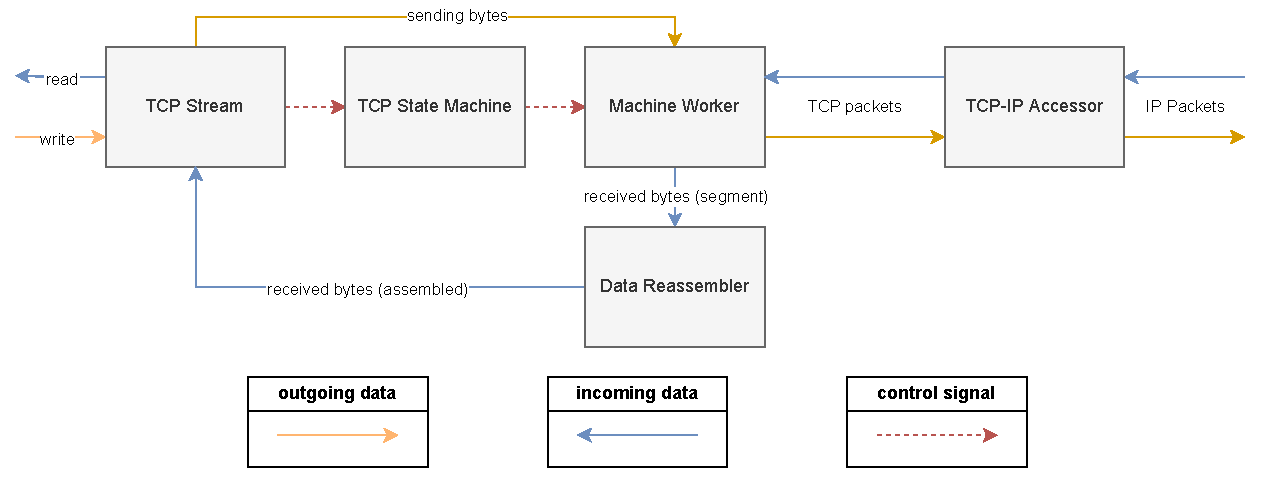
\includegraphics[width=\columnwidth]{./figures/tcpstream.pdf}}
    \caption{the structure of TCP Stream}
    \label{tcpstream}
  \end{center}
\end{figure}
\begin{figure}[H]
  \begin{center}
    \centerline{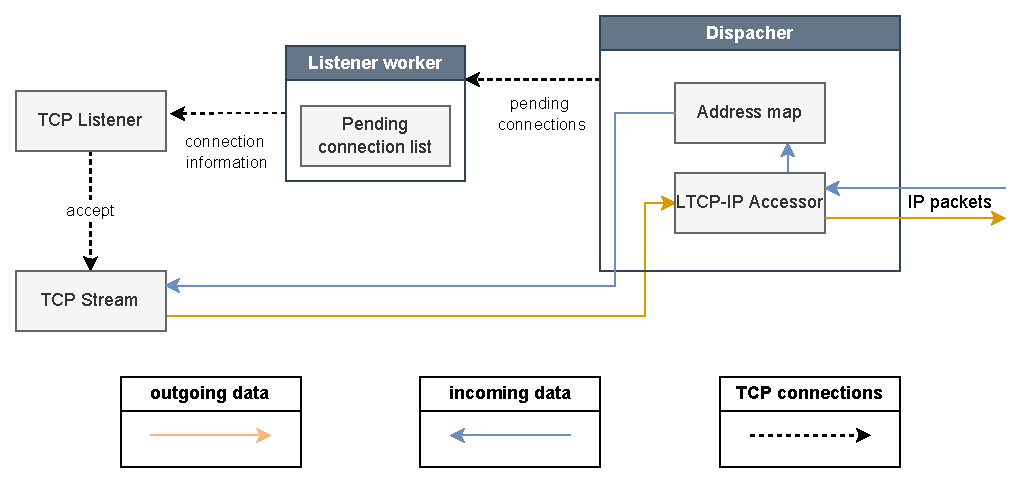
\includegraphics[width=\columnwidth]{./figures/tcplistener}}
    \caption{the structure of TCP Listener}
    \label{tcplistener}
  \end{center}
\end{figure}
As depicted in Figure~\ref{tcpstream}, TCP Stream is composed of five parts.
\begin{itemize}
  \item \textbf{TCP Stream:} The host interacts directly with the TCP Stream. TCP Stream will send the data to the Machine Worker and receive data from Data Reassembler.
  \item \textbf{TCP State Machine} will handle the control signal (such as connecting to the remote or closing the connection) from TCP Stream and send them to the Machine Worker. TCP State Machine is also responsible for releasing the resources after the host drops TCP Stream.
  \item \textbf{Machine Worker} handles the state transition of the TCP. It will also pack the data from the TCP stream, send them to the TCP-IP Accessor, unpack the incoming TCP packets, and send the unpacked bytes to Data Reassmebler.
  \item \textbf{TCP-IP Accessor} is the bridge between the network layer and the transport layer. It packs the TCP packets into IP Packets, periodically receives IP packets, and sends the unpacked TCP packets to the Machine Worker.
  \item \textbf{ Data Reassembler} receives the byte segment from the Machine Worker and reassembles them according to the TCP sequence number. The reassembled bytes will then be sent to the TCP Stream for the host to read.
\end{itemize}
\subsubsection{TCP Listener}

As shown in Figure~\ref{tcplistener}, TCP Listener is composed of three parts:
\begin{itemize}
  \item \textbf{TCP Listener} responds to the host's request. It will ask the Listener Worker for information on the incoming connection if it tries to accept a connection. The created TCP Stream will change its TCP-IP accessor to the Dispatcher.
  \item \textbf{Listener Woker} receives the connection from the Dispatcher and temporarily stores it for the TCP Listener.
  \item \textbf{Dispacher} owns an LTCP-IP Accessor to communicate with the IP server. On receiving the IP packet, it will dispatch the inner TCP packet according to its Address map. If the TCP is an SYN packet, it will create a new entry in the Address Map and send the information to the Listener Worker. On receiving TCP packets from the TCP Stream, it will pack them into IP packets and forward them to the IP server.
\end{itemize}
The TCP Listener is capable of handling multiple connections at the same time.

\section{Application Layer}
\lipsum[17]
\subsection{File Transfer Protocol}
\lipsum[18]
\subsection{Tunneling}
\lipsum[19]

\section{Conclusion}
\lipsum[20]

\section*{Acknowledgement}
We would like to express our sincere gratitude to our course teacher Zhice Yang, for providing the knowledge and guidance to complete this project. We would also like to thank our colleagues, Wenchao Li and Jiajun Cheng. Their valuable feedback, suggestions, and support have been instrumental in completing this project.

We would also like to thank the Rust community for providing us with the resources, libraries and platform to develop this project. In completing this project, we used the following libraries (listed in alphabetical order):
\begin{itemize}
  \item az: Casts and checked casts.
  \item bitvec: Addresses memory by bits, for packed collections and bitfields
  \item clap: A simple to use, efficient, and full-featured Command Line Argument Parser.
  \item crc: Rust implementation of CRC(16,32,64) with support for various standards.
  \item crossbeam: Tools for concurrent programming.
  \item crossbeam-channel: Multi-producer multi-consumer channels for message passing.
  \item cordic: Special functions for fixed-point numbers using the CORDIC method.
  \item console: A terminal and console abstraction for Rust.
  \item cpal: A low-level cross-platform audio I/O library.
  \item fixed: Fixed-point numbers.
  \item hound: A wave encoding and decoding library.
  \item log: A lightweight logging facade for Rust.
  \item env\_logger: A logging implementation for log which is configured via an environment variable.
  \item parking\_lot: More compact and efficient implementations of the standard synchronization primitives
  \item pnet: Cross-platform, low level networking using the Rust programming language.
  \item postcard: A no\_std + serde compatible message library for Rust.
  \item rand: Random number generators and other randomness functionality.
  \item reed-solomon-erasure: Rust implementation of Reed-Solomon erasure coding.
  \item rustfft: High-performance FFT library written in pure Rust.
  \item serde: A generic serialization/deserialization framework
  \item socket2:Utilities for handling networking sockets with a maximal amount of configuration possible intended.
\end{itemize}
We have great respect for their developers and maintainers.
% \bibliographystyle{sdss2020} % Please do not change the bibliography style
% \bibliography{reference}

\end{document}
